\chapter{SCADA}
\label{ch:scada}

%Finalmente y para resumir la evolución del proyecto hasta este punto
Para continuar en el desarrollo es necesario analizar los pasos antes descriptos para la construcción
de la planta. De esta manera, en el capitulo \ref{ch:DisenoEnsamblado} detallamos el sistema 
físico, lo que nos conduce a describir en el capitulo \ref{ch:tablero} el sistema eléctrico y
electrónico que anima a la planta, continuando en el capitulo \ref{ch:progPLC} con la lógica
que regula al sistema completo por medio del \gls{plc}. 

Como elemento final del \gls{pfe} se diseño y realizo una \gls{hmi} \gls{scada}
mediante P-CIM para Windows con el objetivo de poder manipular la planta/el sistema
sin tener un acceso físico a la misma.

En el siguiente capitulo se detallan cada uno de los pasos para la realización de tal interfaz
así como también la configuración actual. Mediante esta información el lector podrá entender
y por lo tanto modificar en caso de ser necesario el entorno. Este capitulo no esta 
orientado a la operación misma de la planta mediante el \gls{scada} lo cual se detalla en 
\todo{agregar la sección donde se describe la operación mediante el scada}

\section{Introducción a SCADA}
\label{sec:IntroScada}

Aunque un \gls{plc} realiza automáticamente un control pre-programado sobre un proceso, 
no tienen una manera estándar de presentar la información al operador y normalmente se 
distribuyen a lo largo de toda la planta, haciendo difícil recoger los datos de manera 
manual.%para poder concentrarlos

En cambio, los sistemas \gls{scada} obtienen los datos desde el \gls{plc} o desde otros controladores 
por medio de algún tipo de red y de manera automática. Posteriormente esta información 
es combinada y formateada en una base de datos para proporcionar las tendencias, alarmas 
integradas y monitoreo de eventos. Luego la presentación de los datos de plantas, máquinas y 
equipos industriales se realiza mediante una \gls{hmi}. También se pueden 
incluir datos de diagnóstico y manejo de la información así como un cronograma de 
procedimientos de mantenimiento, información logística, esquemas detallados para un sensor 
o máquina en particular o incluso sistemas expertos con guía de resolución de problemas. Es entonces
claro que la utilización de un sistema \gls{scada} reduce fuertemente las tareas asociadas al control
y monitoreo de plantas industriales.

\section{Scada P-CIM}
\label{sec:ScadaPCIM} 
\todo{agregar link para la descarga?}
Para el diseño y desarrollo del sistema \gls{scada} de este \gls{pfe} se utilizó el software 
P-CIM para Windows. El mismo, provee de un ambiente de desarrollo y ejecución de aplicaciones 
\gls{scada}.Así, una ves concretado el diseño el \gls{scada} recopila constantemente información 
de la planta en tiempo real. En la base de datos donde se almacenan, evalúan y generan alarmas 
a partir de estos datos.Finalmente, mediante la \gls{hmi} se brinda la información y se pueden 
emitir instrucciones a los \gls{plc} en la planta. 

Dentro de sus características se encuentran:
\begin{itemize}
 \item Corre en todas las plataformas MS-Windows actuales.
 \item Soporte de un gran número de diferentes \gls{plc} y otros dispositivos periféricos.
 \item Drivers para diversos buses de comunicación.
 \item Provee herramientas para el desarrollo de \gls{hmi} inteligentes 
 \item Seguimiento de los procesos de la planta y las actividades de los operadores
 \item Entorno para monitorear alarmas y eventos en toda la extensión de la planta
\end{itemize}


\subsection{Estructura de P-CIM}
\label{sec:CapasPrograma}
Como se puede observar en la figura\todo{agregar capas de abstraccion} la estructura de P-CIM 
para Windows se divide en tres grandes capas:
\begin{itemize}
 \item Capa de Comunicación: Se encarga de la comunicación entre el \gls{plc} y la PC.
 \item Capa de Procesamiento de Datos: Donde se lleva a cabo la mayor parte del procesamiento 
 de datos, registro histórico y manejo de alarmas.
 \item Capa de aplicación: Presenta la información, interactúa con el operador y realiza 
 los controles de alto nivel y de programación.
\end{itemize}

El trabajo coordinado se resume en que la información de campo del PLC llega al \gls{scada} a 
través de la capa de comunicación. Esta se transfiere a la Capa de Procesamiento de Datos (Servidor 
de la Base de Datos o Database Server) donde se analiza. La capa de aplicación la procesa y envía 
hacia la \gls{hmi}. De esta manera el funcionamiento conjunto de cada una de estas capas permite 
al sistema \gls{scada} funcionar de manera correcta y con las prestaciones antes mencionadas.


\section{Desarrollo de la aplicacion SCADA con P-CIM}

A continuación, se detalla la aplicación \gls{scada} desarrollada para este \gls{pfe} en el software
P-CIM para Windows. Su exposición esta dividida de acuerdo a la estructura en capas del programa,como 
se describió en la sección \ref{sec:CapasPrograma}.

\subsection{Capa de comunicación}
\label{subsec:CapaComunicacion}

El primer paso para el desarrollo de un sistema \gls{scada} es lograr la comunicación por medio
de algún bus con el \gls{plc} que controla la planta, formando así la capa de comunicación. 
En nuestro caso se utilizó el protocolo de comunicaciones Modbus. A continuación se detalla el 
proceso de configuración y puesta en marcha del bus. 

\subsubsection{Modbus}
Modbus es un protocolo de comunicaciones diseñado en 1979 por Modicon para su gama de 
controladores lógicos programables (PLCs). Modbus esta situado en la capa de aplicación 
del modelo \gls{osi} con una arquitectura maestro/esclavo o cliente/servidor usándose 
para la conexión entre un computador corriendo un software \gls{scada} y un o varios 
\gls{plc}. Existen versiones del protocolo Modbus para puerto serie y Ethernet (Modbus/TCP).

Simple y robusto, se ha convertido en un protocolo de 
comunicaciones estándar de facto en la industria, gozando de una gran disponibilidad para la 
conexión de dispositivos electrónicos industriales. Las principales razones para el uso de Modbus 
en entornos industriales son:
\begin{itemize}
 \item Fue desarrollado para aplicaciones industriales.
 \item Su implementación es fácil y requiere poco mantenimiento.
 \item Maneja bloques de datos sin suponer restricciones a los vendedores.
 \item Permite la comunicación entre múltiples dispositivos en la misma red. Aprox. 240
 \item De código abierto y libre de regalías.%openly published and royalty-free
\end{itemize}
El desarrollo y actualización del protocolo Modbus ha sido manejado por Modbus Organization desde
abril del 2004 cuando Schneider Electric transfirió los derechos a esta organización.

\subsubsection{Instalación Driver Modbus}
\todo{Agregar link para la descarga?}
Para realizar la instalación del driver de comunicaciones Modbus seguimos los siguientes pasos: 

\begin{enumerate}
 \item Elija $Setup~de~P-CIM$ del grupo de aplicaciónes P-CIM para Windows 32.
Aparecerá en la pantalla la ventana de $Setup~de~P-CIM$.\todo{agregar captura de pantalla}
\item Elija $Install~P-CIM~Driver$. La ventana de diálogo de instalación del Driver de P-
CIM, le pedirá que indique el directorio de origen.
\item Oprima Browse, seleccione el directorio de origen del driver para Modbus en el disco 
C:\todo{agregar ruta completa}, oprima OK y luego Next
\item El Setup de P-CIM despliega la ventana de diálogo de Bienvenida.
\item Para continuar, oprima NEXT. El Setup de P-CIM despliega la ventana de
diálogo de Propiedades del Driver de P-CIM para Windows 32, indicando los
detalles del driver a ser instalado.
\item Elija el/los proyecto(s) en los que Ud. desea instalar el driver o bien seleccione
All (todos) y oprima Next.
\item El Setup de P-CIM procede a efectuar la instalación y finalmente muestra este mensaje: 
“la instalación del driver se ha completado”. Oprima OK para que desaparezca el cuadro de diálogo.
\end{enumerate}

\todo{Agregar capturas de pantalla para la instalacion del software}

\subsubsection{Configuracion Driver Modbus}
Una ves que el driver de Modbus para PCIM se ha instalado correctamente procedemos a realizar su 
configuración para lograr la comunicación entre el PLC y la computadora de control. Esta tarea se
divide en dos partes: 
\begin{itemize}
 \item Asociar el driver con un puerto P-CIM:\\
 P-CIM para Windows 32 soporta 255 puertos lógicos, nombrados de 1 al 255.
 \begin{enumerate}
  \item Elija el Setup de P-CIM del grupo P-CIM para Windows 32.
  \item  Elija el Setup de Comunicación de P-CIM (ALT+M). El Setup de P-CIM
despliega la ventana de diálogo “Communication Setup” de P-CIM.
  \item Para agregar una nueva asociación driver-puerto, elija New (ALT+N) o para
  editar una asociación existente, marque la línea correspondiente y
  elija Edit (ALT+E).
  \item El Setup de P-CIM despliega la ventana de diálogo “Port properties” (propiedades
  de puerto).
  \item Ingrese el número de puerto entre 1 y 255 en la lista de Nombres de Puerto de
  la ventana.
  \item Elija el nombre del driver de la lista de Nombres de Drivers de la ventana (la
  lista contiene nombres de drivers instalados en el proyecto en curso).
  \item En el cuadro elija la notación numérica del bit – octal, decimal o hexadecimal –
  de la lista del Sistema de Numeración del Menor Bit.
  \item Elija la notación usada para referenciar el bit menos significativo – 0 ó 1 – de la
  Lista del Sistema de Numeración del Menor Bit.
  \item Para utilizar el driver en modo emulador, selecciones la casilla de Emulación.
 \end{enumerate}

 \item Establecer los parámetros operativos del puerto.\\
 En esta etapa Ud. define las propiedades de un driver para cada puerto (lógico)
 de P-CIM con el que está asociado.
 \begin{enumerate}
  \item Elegir el Setup de P-CIM del grupo P-CIM para Windows 32.
  \item Elegir el Setup de Comunicación de P-CIM (ALT+M). El Setup de P-CIM
  despliega la ventana de diálogo Communication Setup de P-CIM.
  \item Marque la línea correspondiente en el cuadro de Puertos Asignados y elija
  Propiedades (ALT+P).
  \item El Setup de P-CIM despliega la ventana de diálogo driver específico.
  Proceda como se indica en la guía de ese driver determinado.
 \end{enumerate} 
\end{itemize}

\subsubsection{Verificación comunicación}
En este punto podemos verificar que la comunicación entre el PLC y la
computadora de control se haya establecido. Para monitorear el estado 
de la comunicación podemos utilizar las siguientes herramientas:
\begin{itemize}
 \item Sumario de Alarmas(Alarm Summary):\\
 Despliega mensajes del Sistema de Arranque, uno de los cuales es: “MODBUS
  Driver successfully loaded” indicando que el driver halló la tabla de comunicación y
  fue exitosamente cargado.
 \item Monitor de Datos (Datascope):\\
 Para monitorear el estado de la comunicación,
  debe ingresar en el Monitor de Datos cualquier dirección de PLC que esté definida
  en la tabla de Polling. Al hacerlo, Ud. tendrá un valor por la dirección que insertó,
  indicando que la comunicación está funcionando, o bien recibirá un cero, y
  después de un momento se desplegará un mensaje en la ventana de Resumen
  de Alarma, indicando que la comunicación falló. Veasé la sec\todo{seccion de las direcciones}
  para mas información acerca de las direcciones del PLC y la base de datos.
\end{itemize}


\subsection{Capa de procesamiento}
\label{subsec:CapaProcesamiento}
Una ves que hemos verificado que se ha establecido la comunicación con el \gls{plc}, 
nos ocuparemos de la base de datos de P-CIM para Windows. Esta se encarga de recuperar, 
almacenar y procesar la información de tiempo real e histórica de los controladores, 
dispositivos periféricos y variables internas, por esta razón conforma la capa de 
procesamiento.

La base de datos esta formada por elementos llamados bloques que son utilizados para:
\begin{itemize}
 \item Proporcionar una interfase con el operador.
 \item Generar alarmas.
 \item Intercambiar información.
 \item Registrar información a ser usada en las tendencias.
 \item Convertir información en unidades de ingeniería.
\end{itemize}
La creación de los bloques de la base de datos es un paso importante que debería
ser llevado a cabo después de establecer las comunicaciones.


\subsubsection{Diseño de la base de datos}
Para configurar y editar la base de datos se utiliza el programa $Editor~de~la~Base~de~Datos$.
Al crear la base de datos, se deben tener en cuenta los siguientes puntos:
\begin{itemize}
 \item Tipo de Bloque:\\Existen 8 tipos de bloques de base de datos para el
manejo de 4 tipos básicos de datos: analógicos (enteros o reales), digitales (un
solo bit), string o cadena de caracteres (veinte palabras de 16 bits) y
alarmas (en grupos de 16 bits)
\item Tiempo de Escrutinio (scan) y de Fase:\\Que son respectivamente:
  \begin{itemize}
  \item El intervalo entre sucesivos procesamientos del bloque.
  \item El tiempo inicial de demora entre la carga de la base de datos hasta el primer
  procesamiento del bloque.
  \end{itemize}
  Ambos en el orden de 1-255 unidades donde la unidad de tiempo por defecto es un segundo.
\item Alarmas:\\Las alarmas pueden ser definidas para los bloques de Valor Analógico, Valor
Digital, de Cálculo y Booleanos.
\item Tendencias en tiempo real a corto plazo (S.T.) e Histórica (H.T.):son el número de lecturas 
  (0-255) a ser promediadas para cada punto 
  \begin{itemize}
  \item en un gráfico de tendencia en tiempo real.
  \item registrado en el archivo de tendencia histórica
  \end{itemize}
  respectivamente.
\item Target y Targetlogic:\\Los bloques del target son campos de la base de datos que reciben valores de
otros bloques de la base de datos.
\item Aseguramiento (Clamping):\\Es utilizado para limitar la salida de un bloque de la base de datos o
la entrada de un control a una especificada amplitud de valores superior/inferior.
\item Inversión:\\ Invierte los valores de la entrada desde el dispositivo y los
valores de la salida hacia el dispositivo.
\end{itemize}

Teniendo en cuenta estos aspectos y las variables definidas en el \gls{plc}(Ver tabla) \todo{agregar la tabla de variables PLCs}
para ser leidas por el \gls{scada} definimos los siguientes 3 tipos de bloques
\begin{itemize}
 \item Analog Read/Write: Información desde/hacia el \gls{plc} a la base de datos. Debemos definir entradas
 a la base de datos con la dirección del espacio de memoria en el \gls{plc} para poder acceder en Lectura/Escritura
 en estos registros.
 \item Analog Emulation: Información hacia/desde el \gls{hmi} del \gls{scada} a la base de datos. Es necesario 
 definir variables internas del \gsl{scada} para ser utilizadas para lectura/escritura de la \gls{hmi}.
 \item Calculation:  Conversiones en unidades de ingeniería o porcentual según sea necesario. 
 Las variables leídas del \gls{plc} estan definidas en una escala de $0~a~4095$ por esta razón deben ser
 convertidas para adaptarse tanto al \gls{plc} como al \gls{hmi} del \gls{scada}.
\end{itemize}
Ahora podemos definir el diseño de nuestra base de datos como se muestra en la tabla\todo{tabla con los bloques DB}

%\begin{figure}[t]
  \centering 
  \resizebox{0.8\textwidth}{!}{
  
  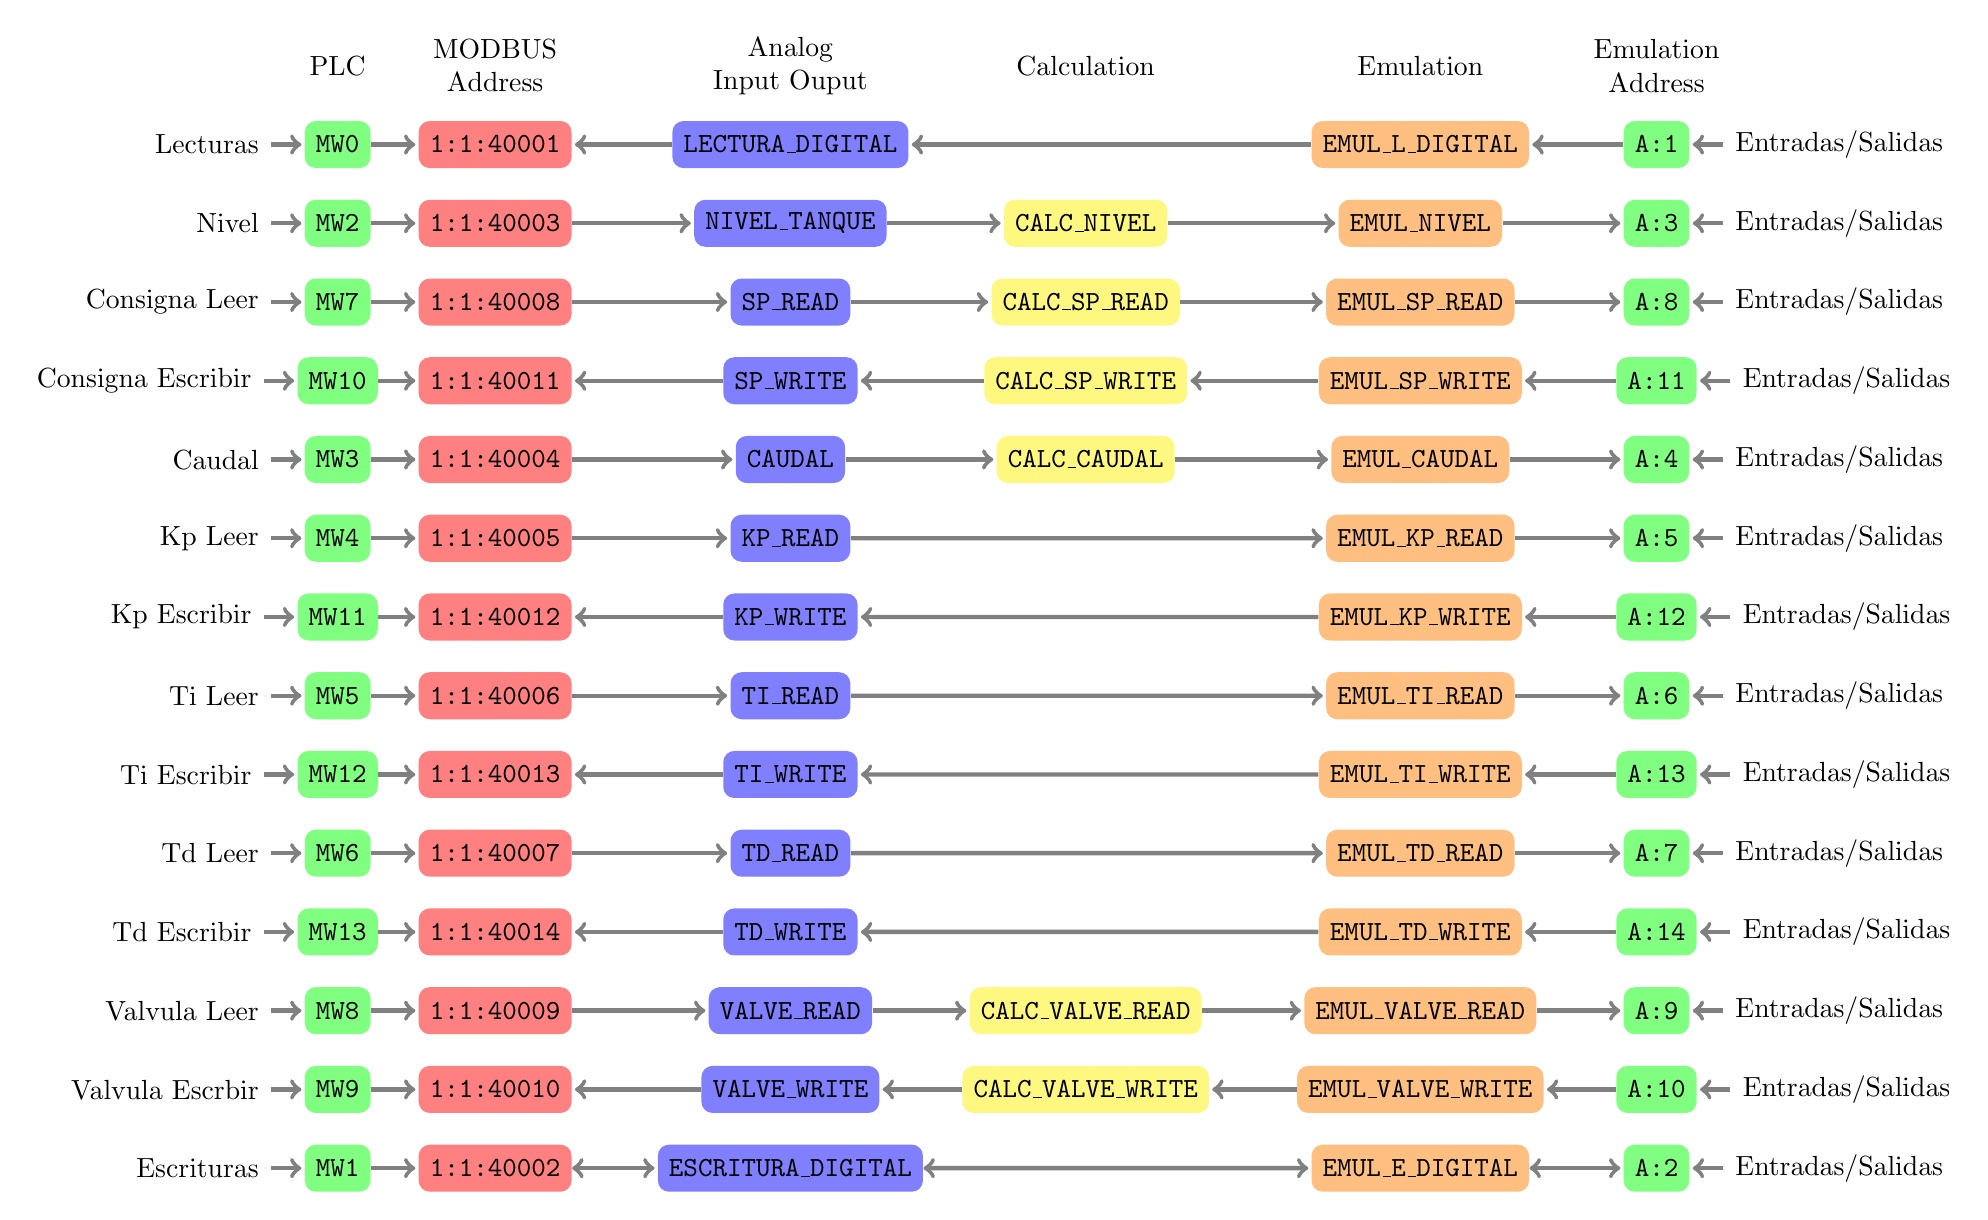
\begin{tikzpicture}[shorten >=1pt,->,draw=black!50]
    \tikzstyle{every pin edge}=[<-,shorten <=1pt, ultra thick]
    \tikzstyle{neuron}=[rectangle,fill=black!25,minimum size=17pt,inner 
sep=4pt, rounded corners]
    \tikzstyle{annot} = [text width=7em, text centered]

    \tikzstyle{plc neuron}=[neuron, fill=green!50];
    \tikzstyle{modbus neuron}=[neuron, fill=red!50, node 
    distance=0.4*5cm];
    \tikzstyle{aio neuron}=[neuron, fill=blue!50, node 
    distance=0.75*5cm];
    \tikzstyle{calc neuron}=[neuron, fill=yellow!50, node 
    distance=0.75*5cm];
    \tikzstyle{emul neuron}=[neuron, fill=orange!50, node 
    distance=0.85*5cm];
    \tikzstyle{emula neuron}=[neuron, fill=green!50, node 
    distance=0.6*5cm];

    % Draw the plc layer nodes
     \node[plc neuron, pin=left:Lecturas] (mw0) at (0,0) 
{\texttt{MW0}};
     \node[plc neuron, pin=left:Nivel] (mw1) at (0,-1) 
{\texttt{MW2}};
     \node[plc neuron, pin=left: Consigna Leer] (mw2) at (0,-2) 
{\texttt{MW7}};
     \node[plc neuron, pin=left: Consigna Escribir] (mw10) at (0,-3) 
{\texttt{MW10}};
     \node[plc neuron, pin=left: Caudal] (mw3) at (0,-4) 
{\texttt{MW3}};
      \node[plc neuron, pin=left: Kp Leer] (mw4) at (0,-5) 
 {\texttt{MW4}};
      \node[plc neuron, pin=left: Kp Escribir] (mw11) at (0,-6) 
 {\texttt{MW11}};
      \node[plc neuron, pin=left: Ti Leer] (mw5) at (0,-7) 
 {\texttt{MW5}};
      \node[plc neuron, pin=left: Ti Escribir] (mw12) at (0,-8) 
 {\texttt{MW12}};
      \node[plc neuron, pin=left: Td Leer] (mw6) at (0,-9) 
 {\texttt{MW6}};
      \node[plc neuron, pin=left: Td Escribir] (mw13) at (0,-10) 
 {\texttt{MW13}};
      \node[plc neuron, pin=left: Valvula Leer] (mw7) at (0,-11) 
 {\texttt{MW8}};
      \node[plc neuron, pin=left: Valvula Escrbir] (mw15) at (0,-12) 
 {\texttt{MW9}};
      \node[plc neuron, pin=left: Escrituras] (mw8) at (0,-13) 
 {\texttt{MW1}};

    %Draw Modbus layer nodes
    \node[modbus neuron, right of=mw0] (40001)  {\texttt{1:1:40001}};
    \node[modbus neuron, right of=mw1] (40002)  {\texttt{1:1:40003}};
    \node[modbus neuron, right of=mw2] (40003)  {\texttt{1:1:40008}};
    \node[modbus neuron, right of=mw3] (40004)  {\texttt{1:1:40004}};
    \node[modbus neuron, right of=mw4] (40005)  {\texttt{1:1:40005}};
    \node[modbus neuron, right of=mw5] (40006)  {\texttt{1:1:40006}};
    \node[modbus neuron, right of=mw6] (40007)  {\texttt{1:1:40007}};
    \node[modbus neuron, right of=mw7] (40008)  {\texttt{1:1:40009}};
    \node[modbus neuron, right of=mw8] (40009)  {\texttt{1:1:40002}};
    \node[modbus neuron, right of=mw10] (40011)  {\texttt{1:1:40011}};
    \node[modbus neuron, right of=mw11] (40012)  {\texttt{1:1:40012}};
    \node[modbus neuron, right of=mw12] (40013)  {\texttt{1:1:40013}};
    \node[modbus neuron, right of=mw13] (40014)  {\texttt{1:1:40014}};
    \node[modbus neuron, right of=mw15] (40016)  {\texttt{1:1:40010}};
     
    %Draw Analog Input Output layer nodes
    \node[aio neuron, right of=40001] (io)  {\texttt{LECTURA\_DIGITAL}};
    \node[aio neuron, right of=40002] (niv)  {\texttt{NIVEL\_TANQUE}};
    \node[aio neuron, right of=40003] (spr)  {\texttt{SP\_READ}};
    \node[aio neuron, right of=40004] (caudal)  {\texttt{CAUDAL}};
    \node[aio neuron, right of=40005] (kpr)  {\texttt{KP\_READ}};
    \node[aio neuron, right of=40006] (tir)  {\texttt{TI\_READ}};
    \node[aio neuron, right of=40007] (tdr)  {\texttt{TD\_READ}};
    \node[aio neuron, right of=40008] (vr)  {\texttt{VALVE\_READ}};
    \node[aio neuron, right of=40009] (md)  {\texttt{ESCRITURA\_DIGITAL}};
    \node[aio neuron, right of=40011] (spw)  {\texttt{SP\_WRITE}};
    \node[aio neuron, right of=40012] (kpw)  {\texttt{KP\_WRITE}};
    \node[aio neuron, right of=40013] (tiw)  {\texttt{TI\_WRITE}};
    \node[aio neuron, right of=40014] (tdw) {\texttt{TD\_WRITE}};
    \node[aio neuron, right of=40016] (vw)  {\texttt{VALVE\_WRITE}};

    %Draw Calculation
    \node[calc neuron, right of=niv] (cniv) {\texttt{CALC\_NIVEL}};
    \node[calc neuron, right of=spr] (cspr) {\texttt{CALC\_SP\_READ}};
    \node[calc neuron, right of=spw] (cspw) {\texttt{CALC\_SP\_WRITE}};
    \node[calc neuron, right of=caudal] (ccaudal) {\texttt{CALC\_CAUDAL}};
    \node[calc neuron, right of=vr] (cvr) {\texttt{CALC\_VALVE\_READ}};
    \node[calc neuron, right of=vw] (cvw) {\texttt{CALC\_VALVE\_WRITE}};
    
    %Draw ResultCalculation
    \node[emul neuron, right of=cniv] (eniv) {\texttt{EMUL\_NIVEL}};
    \node[emul neuron, right of=cspr] (espr) {\texttt{EMUL\_SP\_READ}};
    \node[emul neuron, right of=cspw] (espw) {\texttt{EMUL\_SP\_WRITE}};
    \node[emul neuron, right of=ccaudal] (ecaudal) {\texttt{EMUL\_CAUDAL}};
    \node[emul neuron, right of=cvr] (evr) {\texttt{EMUL\_VALVE\_READ}};
    \node[emul neuron, right of=cvw] (evw) {\texttt{EMUL\_VALVE\_WRITE}};
    
    %Draw Emulation
    \node[emul neuron] (eio) at (2.75*5cm,0 cm) 
{\texttt{EMUL\_L\_DIGITAL}};
    \node[emul neuron] (ekpr) at (2.75*5cm,-5 cm) 
{\texttt{EMUL\_KP\_READ}};
    \node[emul neuron] (etir) at (2.75*5cm,-7 cm) 
{\texttt{EMUL\_TI\_READ}};
    \node[emul neuron] (etdr) at (2.75*5cm,-9 cm) 
{\texttt{EMUL\_TD\_READ}};
    \node[emul neuron] (emd) at (2.75*5cm,-13 cm) 
{\texttt{EMUL\_E\_DIGITAL}};
    \node[emul neuron] (ekpw) at (2.75*5cm,-6 
cm){\texttt{EMUL\_KP\_WRITE}};
    \node[emul neuron] (etiw) at (2.75*5cm,-8 cm) 
{\texttt{EMUL\_TI\_WRITE}};
    \node[emul neuron] (etdw) at (2.75*5cm,-10 cm) 
{\texttt{EMUL\_TD\_WRITE}};

    %Draw internal variables
   \node[emula neuron, pin=right:Entradas/Salidas,right of=eio] (a1) 
  {\texttt{A:1}};
  \node[emula neuron, pin=right:Entradas/Salidas,right of=eniv] (a2) 
  {\texttt{A:3}};
  \node[emula neuron, pin=right:Entradas/Salidas,right of=espr] (a3) 
  {\texttt{A:8}};
  \node[emula neuron, pin=right:Entradas/Salidas,right of=espw] (a11) 
  {\texttt{A:11}};
  \node[emula neuron, pin=right:Entradas/Salidas,right of=ecaudal] (a4) 
  {\texttt{A:4}};
  \node[emula neuron, pin=right:Entradas/Salidas,right of=ekpr] (a5) 
  {\texttt{A:5}};
  \node[emula neuron, pin=right:Entradas/Salidas,right of=ekpw] (a12) 
  {\texttt{A:12}};
  \node[emula neuron, pin=right:Entradas/Salidas,right of=etir] (a6) 
  {\texttt{A:6}};
  \node[emula neuron, pin=right:Entradas/Salidas,right of=etiw] (a13) 
  {\texttt{A:13}};
  \node[emula neuron, pin=right:Entradas/Salidas,right of=etdr] (a7) 
  {\texttt{A:7}};
  \node[emula neuron, pin=right:Entradas/Salidas,right of=etdw] (a14) 
  {\texttt{A:14}};
  \node[emula neuron, pin=right:Entradas/Salidas,right of=evr] (a8) 
  {\texttt{A:9}};
  \node[emula neuron, pin=right:Entradas/Salidas,right of=evw] (a16) 
  {\texttt{A:10}};
  \node[emula neuron, pin=right:Entradas/Salidas,right of=emd] (a9) 
  {\texttt{A:2}};

   
  % Connect every node 
  %PLC -> MODBUS
  \path (mw0) edge[ultra thick] (40001); 
  \path (mw1) edge[ultra thick] (40002); 
  \path (mw2) edge[ultra thick] (40003);
  \path (mw3) edge[ultra thick] (40004); 
  \path (mw4) edge[ultra thick] (40005); 
  \path (mw5) edge[ultra thick] (40006); 
  \path (mw6) edge[ultra thick] (40007); 
  \path (mw7) edge[ultra thick] (40008); 
  \path (mw8) edge[ultra thick] (40009);
  \path (mw10) edge[ultra thick] (40011); 
  \path (mw11) edge[ultra thick] (40012); 
  \path (mw12) edge[ultra thick] (40013);
  \path (mw13) edge[ultra thick] (40014); 
  \path (mw15) edge[ultra thick] (40016); 

  %MODBUS -> Analog IO
  \path (io) edge[ultra thick] (40001);
  \path (40002) edge[ultra thick] (niv); 
  \path (40003) edge[ultra thick] (spr);
  \path (40004) edge[ultra thick] (caudal);
  \path (40005) edge[ultra thick] (kpr);
  \path (40006) edge[ultra thick] (tir);
  \path (40007) edge[ultra thick] (tdr); 
  \path (40008) edge[ultra thick] (vr);
  \path (40009) edge[<->,ultra thick] (md); 
  \path (spw) edge[ultra thick] (40011); 
  \path (kpw) edge[ultra thick] (40012);
  \path (tiw) edge[ultra thick] (40013); 
  \path (tdw) edge[ultra thick] (40014);
  \path (vw) edge[ultra thick] (40016); 

  %Analog -> Calc
  \path (niv) edge[ultra thick] (cniv);
  \path (spr) edge[ultra thick] (cspr);
  \path (cspw) edge[ultra thick] (spw);
  \path (caudal) edge[ultra thick] (ccaudal);
  \path (vr) edge[ultra thick] (cvr);
  \path (cvw) edge[ultra thick] (vw);

  %Calc -> Emulation
  \path (cniv) edge[ultra thick] (eniv);
  \path (cspr) edge[ultra thick] (espr);
  \path (espw) edge[ultra thick] (cspw);
  \path (ccaudal) edge[ultra thick] (ecaudal);
  \path (cvr) edge[ultra thick] (evr);
  \path (evw) edge[ultra thick] (cvw); 
  
  %Analog IO -> Emulation
  \path (eio) edge[ultra thick] (io);
  \path (kpr) edge[ultra thick] (ekpr);
  \path (ekpw) edge[ultra thick] (kpw);
  \path (tir) edge[ultra thick] (etir);
  \path (etiw) edge[ultra thick] (tiw);
  \path (tdr) edge[ultra thick] (etdr);
  \path (etdw) edge[ultra thick] (tdw);
  \path (md) edge[<->,ultra thick] (emd);

  %Emulation -> Address
  \path (a1) edge[ultra thick] (eio);
  \path (eniv) edge[ultra thick] (a2);
  \path (espr) edge[ultra thick] (a3);
  \path  (a11) edge[ultra thick] (espw);
  \path (ecaudal) edge[ultra thick] (a4);
  \path (ekpr) edge[ultra thick] (a5);
  \path  (a12) edge[ultra thick] (ekpw);
  \path (etir) edge[ultra thick] (a6);
  \path  (a13) edge[ultra thick] (etiw);
  \path (etdr) edge[ultra thick] (a7);
  \path (a14) edge[ultra thick] (etdw);
  \path (evr) edge[ultra thick] (a8);
  \path (a16) edge[ultra thick] (evw);
  \path (emd) edge[<->,ultra thick] (a9);
  

 
  % Annotate the layers
  \node[annot,above of=mw0, node distance=1cm] (plc) {PLC};
  \node[annot,above of=40001, node distance=1cm] (modbus) {MODBUS Address};
  \node[annot,above of=io, node distance=1cm] (aio) {Analog Input Ouput};
  \node[annot,right of=aio, node distance=0.75*5cm] (calc) {Calculation};
  \node[annot,above of=eio, node distance=1cm] (emul) {Emulation};
  \node[annot,above of=a1, node distance=1cm] (emula) {Emulation Address};

\end{tikzpicture}
  }

\end{figure}


\subsubsection{Creación de los bloques de la base de datos}

A continuación se muestran los pasos necesarios para la creación de un elemento de la base de datos.
\begin{enumerate}
 \item Active P-CIM para Windows utilizando el Startup de P-CIM.
 \item En el directorio de P-CIM oprima el icono del Editor de la Base de Datos.
 \item Oprima la tecla Add. El Editor de la Base de Datos despliega la ventana de
  especificaciones de Valor Analógico.
 \item  Ingrese el nombre y complete los campos que correspondan en cada bloque. No se han utilizado
 el resto de las opciones que presenta la base de datos excepto aquellos que fueron expresados anteriormente 
 en la tabla \todo{agregar tabla}
 \item Oprima la tecla OK para regresar al directorio del Bloque.
 \item Oprima la tecla Save DB para guardar la Base de Datos.
\end{enumerate}

Ahora podemos controlar el funcionamiento del bloque recién configurado de la siguiente manera:
\begin{enumerate}
 \item Abra el Datascope (Monitor de Datos), con un doble click sobre su icono en el
 directorio de P-CIM.
 \item Escriba el nombre de alguno de los bloques antes definidos  y en otro item su
 dirección.
 \item Se debe poder observar en ambos el mismo valor leído(en caso de registros de lectura) o el 
 mismo valor al escribir en uno u otro de los items.
\end{enumerate}
Si esta prueba nos ha dado los resultados esperados podemos estar seguros que nuestros bloques se encuentran 
bien configurados y podemos proseguir con el desarrollo de nuestro sistema \gls{scada}.


\subsection{Capa de aplicación}
\label{subsec:CapaAplicacion}
La tercer y última capa del sistema \gls{scada} es la capa de aplicación. Esta será utilizada en nuestro 
\gls{pfe} unicamente como \gls{hmi}. Para el desarrollo de la interfaz gráfica definimos un documento 
gráfico creado con el Editor de Animaciones (Animation Editor). Finalmente, mediante el Servidor de 
Pantallas (Operator Workstation) se pone en marcha el sistema. A continuación se presentan el desarrollo 
y descripción de la pantalla realizada mediante las herramientas gráficas provistas por P-CIM para Windows

Incluye ilustraciones, indicadores y controles emulando un panel de control real
pero con muchos más elementos. Actúa como interfase entre el operador y la planta.


\subsubsection{Diseño de una pantalla}
El primer paso en el diseño de un pantalla es la definición de requerimientos con los que debemos cumplir. 
Estos se resumen en:
\begin{itemize}
 \item Encendido y Parada de la planta.
 \item Visualización del estado actual de la planta: Niveles, caudal, bombas encendidas, etc

 \item Control Manual
 \begin{itemize}
  \item Encender las bombas de manera independiente.
  \item Controlar la abertura de la válvula
 \end{itemize}

 \item Control Automático
 \begin{itemize}
  \item Visualizar el seguimiento de la consigna.
  \item Visualizar/Definir la consigna
  \item Visualizar/Definir las constantes del controlador
 \end{itemize}
\end{itemize}

Ahora mediante el Editor de Animaciones procedemos a producir y definir las características 
funcionales de la pantalla  que correrá en el Operator Workstation. Mediante las 
características antes especificadas se obtuvo el resultado que se observa 
en la figura \todo{agregar figura hmi}. 

Para dicha interfaz se procedió en el siguiente orden
\begin{enumerate}
 \item Iniciar el Editor de Animaciones. Elegir el icono de la carpeta de P-CIM. Aparece un pantalla 
 sin nombre. Guarde el archivo asignandole un nombre.
 \item Crear la ilustración básica.\\
    Use el Editor de Animaciones para  dibujar sus propios gráficos 
    o insertar objetos gráficos ya creados de la biblioteca de ClipArt.Los objetos gráficos insertados 
    desde el ClipArt pueden tratarse como cualquier otro objeto gráfico y ser movidos, redimensionados, 
    editados y asignados con propiedades.
    Para seleccionar un objeto de ClipArt:
    \begin{enumerate}
      \item Elegir "’ClipArt” en el menú File, luego elegir la categoría en el submenú o elegir el botón 
      categoría de la caja de ClipArt.
      \item Hacer click en el objeto para seleccionarlo.
      \item Hacer click nuevamente sobre el objeto seleccionado, mantener presionada la tecla CTRL y 
      el botón izquierdo del mouse, arrastrar el objeto hasta el lugar deseado en el pantalla y soltar 
      el botón del mouse y la tecla CTRL. La ventana de ClipArt se cierra tan pronto Ud. comienza a 
      arrastrar el objeto.
    \end{enumerate}

 \item Animar la ilustración.\\
      Para animar un objeto gráfico se debe seleccionar el objeto y especificar una o
      más propiedades de la Lista de Propiedades (Properties List).
      Para comenzar a animar un objeto
      \begin{enumerate}
	\item Seleccionar el objeto (click izquierdo del mouse); por ejemplo un rectángulo. El
	Editor de Animaciones le coloca marcas al objeto.
	\item Elegir Properties List (Lista de Propiedades) 
      \end{enumerate}
      Las propiedades están divididas en tres
      categorías principales: Controls, Indicators, y Special 
      (controles, indicadores y especiales).
      \begin{itemize}
	\item  Controls: especifica una entrada de datos la cual puede estar dada por 
	casillas de entrada de datos, botones que inician acciones, o
	potenciómetros que permiten fijar valores analógicos.
	\item Indicators: Usados para crear presentaciones textuales, de color
	y gráficas de los datos, en estos los contenidos, posición, color y
	tamaño cambian en función del valor de los datos.
	\item Special: esta categoría es usada para especificar Gráficos de Tendencia o
	“Medidores de Desviación”.
      \end{itemize}
      Un signo de visto en una casilla de propiedades significa que ésta es la propiedad
      asignada al objeto gráfico. Luego aparece otra ventana de diálogo:
      donde se debe completar (Servidor, Tópico e Item) para cada
      propiedad que especifique (excepto para el botón). Esto designa
      respectivamente el origen de los datos mostrados por el indicador o 
      el destino de los datos escritos por el objeto de control.
      
 \item Probar los resultados en el Operator Workstation.\\
      Para poder probar el funcionamiento de nuestra \gls{hmi} procedemos de la siguiente manera:
      \begin{enumerate}
       \item 
      \end{enumerate}

\end{enumerate}












Diseño y Requerimientos del Pantalla
Supóngase que el depósito de A en el edificio B se usa para almacenar flores de
exportación. Almacenar flores requiere condiciones especiales, como iluminación y
temperatura. 


\section{Ejecución}
\label{sec:Ejecucion}

Una ves que han sido configuradas cada una de las partes podemos utilizar nuestro sistema SCADA.

